\chapter{时间复杂度}

\index{time complexity}

算法的效率在算法竞赛中十分重要。通常，设计一个能缓慢解决问题的算法并不困难，真正的挑战在于构造快速算法。如果算法太慢，就只能得到部分分数，甚至完全无法得分。

算法的\key{时间复杂度}估计该算法处理某个输入时所需的时间。其思想是用一个以输入规模为参数的函数来表示效率。通过计算时间复杂度，我们无需实现算法就能判断它是否足够快。

\section{计算规则}

算法的时间复杂度记作 $O(\cdots)$，其中省略号表示某个函数。变量 $n$ 通常表示输入规模。例如，若输入是一个数值数组，则 $n$ 表示数组大小；若输入是一个字符串，则 $n$ 表示字符串长度。

\subsubsection*{循环}

算法运行缓慢的常见原因之一，是其中包含许多遍历输入的循环。嵌套循环越多，算法就越慢。如果有 $k$ 层嵌套循环，时间复杂度就是 $O(n^k)$。

例如，以下代码的时间复杂度为 $O(n)$：
\begin{lstlisting}
for (int i = 1; i <= n; i++) {
    // code
}
\end{lstlisting}

而以下代码的时间复杂度为 $O(n^2)$：
\begin{lstlisting}
for (int i = 1; i <= n; i++) {
    for (int j = 1; j <= n; j++) {
        // code
    }
}
\end{lstlisting}

\subsubsection*{数量级}

时间复杂度并不表示循环内代码执行的精确次数，只表示其数量级。在以下示例中，循环内代码分别执行 $3n$、$n+5$ 和 $\lceil n/2 \rceil$ 次，但每段代码的时间复杂度都是 $O(n)$。

\begin{lstlisting}
for (int i = 1; i <= 3*n; i++) {
    // code
}
\end{lstlisting}

\begin{lstlisting}
for (int i = 1; i <= n+5; i++) {
    // code
}
\end{lstlisting}

\begin{lstlisting}
for (int i = 1; i <= n; i += 2) {
    // code
}
\end{lstlisting}

再看一个例子，以下代码的时间复杂度为 $O(n^2)$：

\begin{lstlisting}
for (int i = 1; i <= n; i++) {
    for (int j = i+1; j <= n; j++) {
        // code
    }
}
\end{lstlisting}

\subsubsection*{多个阶段}

如果算法由若干依次执行的阶段组成，总时间复杂度等于单个阶段中最大的时间复杂度。这是因为最慢的阶段通常就是代码的瓶颈。

例如，以下代码由时间复杂度分别为 $O(n)$、$O(n^2)$ 和 $O(n)$ 的三个阶段组成，因此总时间复杂度为 $O(n^2)$。

\begin{lstlisting}
for (int i = 1; i <= n; i++) {
    // code
}
for (int i = 1; i <= n; i++) {
    for (int j = 1; j <= n; j++) {
        // code
    }
}
for (int i = 1; i <= n; i++) {
    // code
}
\end{lstlisting}

\subsubsection*{多个变量}

有时，时间复杂度取决于多个因素。此时时间复杂度公式中会包含多个变量。

例如，以下代码的时间复杂度为 $O(nm)$：

\begin{lstlisting}
for (int i = 1; i <= n; i++) {
    for (int j = 1; j <= m; j++) {
        // code
    }
}
\end{lstlisting}

\subsubsection*{递归}

递归函数的时间复杂度取决于函数的调用次数和单次调用的时间复杂度，总时间复杂度是这两个量的乘积。

例如，考虑以下函数：
\begin{lstlisting}
void f(int n) {
    if (n == 1) return;
    f(n-1);
}
\end{lstlisting}
调用 $\texttt{f}(n)$ 会产生 $n$ 次函数调用，每次调用的时间复杂度为 $O(1)$，因此总时间复杂度为 $O(n)$。

再考虑以下函数：
\begin{lstlisting}
void g(int n) {
    if (n == 1) return;
    g(n-1);
    g(n-1);
}
\end{lstlisting}
除 $n=1$ 外，每次函数调用都会再产生两次调用。下面考察以参数 $n$ 调用 $g$ 时的情况。下表列出了这一次调用所产生的全部函数调用：
\begin{center}
\begin{tabular}{rr}
函数调用 & 调用次数 \\
\hline
$g(n)$ & 1 \\
$g(n-1)$ & 2 \\
$g(n-2)$ & 4 \\
$\cdots$ & $\cdots$ \\
$g(1)$ & $2^{n-1}$ \\
\end{tabular}
\end{center}
由此可知，时间复杂度为
\[1+2+4+\cdots+2^{n-1} = 2^n-1 = O(2^n).\]

\section{复杂度类别}

\index{complexity classes}

下面列出算法中常见的时间复杂度：

\begin{description}
\item[$O(1)$]
\index{constant-time algorithm}
\key{常数时间}算法的运行时间与输入规模无关。典型的常数时间算法是直接用公式计算答案。

\item[$O(\log n)$]
\index{logarithmic algorithm}
\key{对数}算法通常在每一步把输入规模减半。此类算法的运行时间是对数级的，因为 $\log_2 n$ 等于把 $n$ 不断除以 2 直至得到 1 所需的次数。

\item[$O(\sqrt n)$]
\key{平方根算法}比 $O(\log n)$ 慢，但比 $O(n)$ 快。平方根具有一个特殊性质：$\sqrt n=n/\sqrt n$，因此在某种意义上，$\sqrt n$ 位于输入规模的中间位置。

\item[$O(n)$]
\index{linear algorithm}
\key{线性}算法以常数次遍历整个输入。这通常是可能达到的最佳时间复杂度，因为报告答案之前一般至少要访问每个输入元素一次。

\item[$O(n \log n)$]
这种时间复杂度往往意味着算法对输入进行了排序，因为高效排序算法的时间复杂度是 $O(n \log n)$。另一种可能是，算法使用了每次操作耗时 $O(\log n)$ 的数据结构。

\item[$O(n^2)$]
\index{quadratic algorithm}
\key{平方级}算法通常包含两层嵌套循环。可以在 $O(n^2)$ 时间内遍历输入元素的所有二元组。

\item[$O(n^3)$]
\index{cubic algorithm}
\key{立方级}算法通常包含三层嵌套循环。可以在 $O(n^3)$ 时间内遍历输入元素的所有三元组。

\item[$O(2^n)$]
这种时间复杂度往往意味着算法遍历输入元素的所有子集。例如，$\{1,2,3\}$ 的子集为 $\emptyset$、$\{1\}$、$\{2\}$、$\{3\}$、$\{1,2\}$、$\{1,3\}$、$\{2,3\}$ 和 $\{1,2,3\}$。

\item[$O(n!)$]
这种时间复杂度往往意味着算法遍历输入元素的所有排列。例如，$\{1,2,3\}$ 的排列为 $(1,2,3)$、$(1,3,2)$、$(2,1,3)$、$(2,3,1)$、$(3,1,2)$ 和 $(3,2,1)$。

\end{description}

\index{polynomial algorithm}
若算法的时间复杂度至多为 $O(n^k)$，其中 $k$ 是常数，则称该算法是\key{多项式时间}算法。上面除 $O(2^n)$ 和 $O(n!)$ 以外的时间复杂度都是多项式时间。实际中常数 $k$ 通常很小，因此，多项式时间复杂度大体意味着算法是\emph{高效的}。

\index{NP-hard problem}

本书中的大多数算法都是多项式时间算法。然而，许多重要问题目前还没有已知的多项式时间算法，也就是说，人们尚不知道如何高效地解决它们。\key{NP 困难}问题就是一类重要的、尚无已知多项式时间算法的问题\footnote{这一主题的经典著作是 M. R. Garey 和 D. S. Johnson 的 \emph{Computers and Intractability: A Guide to the Theory of NP-Completeness} \cite{gar79}。}。

\section{估算效率}

通过计算算法的时间复杂度，可以在实现之前判断它对当前问题而言是否足够高效。估算的出发点是：现代计算机每秒可以执行数亿次操作。

例如，假设某问题的时间限制为一秒，输入规模为 $n=10^5$。若时间复杂度为 $O(n^2)$，算法将执行大约 $(10^5)^2=10^{10}$ 次操作。这至少需要几十秒，因此该算法似乎太慢，无法解决这个问题。

另一方面，我们也可以根据输入规模\emph{推测}解决该问题所需的时间复杂度。假设时间限制为一秒，下表给出了一些实用估计。

\begin{center}
\begin{tabular}{ll}
输入规模 & 所需时间复杂度 \\
\hline
$n \le 10$ & $O(n!)$ \\
$n \le 20$ & $O(2^n)$ \\
$n \le 500$ & $O(n^3)$ \\
$n \le 5000$ & $O(n^2)$ \\
$n \le 10^6$ & $O(n \log n)$ 或 $O(n)$ \\
$n$ 很大 & $O(1)$ 或 $O(\log n)$ \\
\end{tabular}
\end{center}

例如，当输入规模为 $n=10^5$ 时，题目很可能要求算法的时间复杂度为 $O(n)$ 或 $O(n\log n)$。这一信息排除了会产生更差时间复杂度的方案，使算法设计更容易。

\index{constant factor}

不过，必须记住时间复杂度只是效率的估计，因为它隐藏了\emph{常数因子}。例如，某个 $O(n)$ 算法可能执行 $n/2$ 次操作，也可能执行 $5n$ 次操作。这会显著影响算法的实际运行时间。

\section{最大子数组和}

\index{maximum subarray sum}

解决同一个问题通常有多种算法，它们的时间复杂度可能不同。本节讨论一个经典问题，它有一个直观的 $O(n^3)$ 解法；通过改进算法，又可以把时间降到 $O(n^2)$，甚至 $O(n)$。

给定一个包含 $n$ 个数的数组，我们的任务是计算\key{最大子数组和}，即数组中一段连续元素序列可能取得的最大和\footnote{J. Bentley 的著作 \emph{Programming Pearls} \cite{ben86} 推广了这个问题。}。当数组中可能含有负数时，这个问题才有意义。例如，在数组
\begin{center}
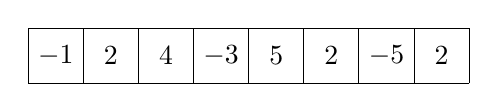
\begin{tikzpicture}[scale=0.7]
\draw (0,0) grid (8,1);

\node at (0.5,0.5) {$-1$};
\node at (1.5,0.5) {$2$};
\node at (2.5,0.5) {$4$};
\node at (3.5,0.5) {$-3$};
\node at (4.5,0.5) {$5$};
\node at (5.5,0.5) {$2$};
\node at (6.5,0.5) {$-5$};
\node at (7.5,0.5) {$2$};
\end{tikzpicture}
\end{center}
\begin{samepage}
中，下面的子数组产生最大和 $10$：
\begin{center}
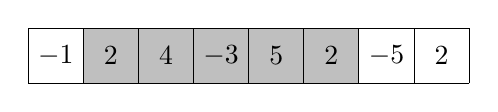
\begin{tikzpicture}[scale=0.7]
\fill[color=lightgray] (1,0) rectangle (6,1);
\draw (0,0) grid (8,1);

\node at (0.5,0.5) {$-1$};
\node at (1.5,0.5) {$2$};
\node at (2.5,0.5) {$4$};
\node at (3.5,0.5) {$-3$};
\node at (4.5,0.5) {$5$};
\node at (5.5,0.5) {$2$};
\node at (6.5,0.5) {$-5$};
\node at (7.5,0.5) {$2$};
\end{tikzpicture}
\end{center}
\end{samepage}

我们允许空子数组，因此最大子数组和始终至少为 $0$。

\subsubsection{算法 1}

一种直接的解法是遍历所有可能的子数组，计算每个子数组的元素和，并维护最大值。以下代码实现了该算法：

\begin{lstlisting}
int best = 0;
for (int a = 0; a < n; a++) {
    for (int b = a; b < n; b++) {
        int sum = 0;
        for (int k = a; k <= b; k++) {
            sum += array[k];
        }
        best = max(best,sum);
    }
}
cout << best << "\n";
\end{lstlisting}

变量 \texttt{a} 和 \texttt{b} 确定子数组的首、尾下标，元素和存入变量 \texttt{sum}。变量 \texttt{best} 保存搜索过程中找到的最大和。

算法包含三层遍历输入的嵌套循环，因此时间复杂度为 $O(n^3)$。

\subsubsection{算法 2}

去掉一层循环就能轻易提高算法 1 的效率。我们可以在子数组右端点移动时同步计算其元素和，得到以下代码：

\begin{lstlisting}
int best = 0;
for (int a = 0; a < n; a++) {
    int sum = 0;
    for (int b = a; b < n; b++) {
        sum += array[b];
        best = max(best,sum);
    }
}
cout << best << "\n";
\end{lstlisting}
修改之后，时间复杂度为 $O(n^2)$。

\subsubsection{算法 3}

令人惊讶的是，这个问题可以在 $O(n)$ 时间内解决\footnote{在 \cite{ben86} 中，这个线性时间算法归功于 J. B. Kadane，因此它有时称为\index{Kadane's algorithm}\key{Kadane 算法}。}，也就是说，只需一层循环。其思想是对每个数组位置，计算以该位置结尾的子数组所能取得的最大和；问题的答案就是这些和中的最大值。

考虑寻找以位置 $k$ 结尾的最大和子数组这一子问题，有两种可能：
\begin{enumerate}
\item 子数组只包含位置 $k$ 上的元素。
\item 子数组由一个以位置 $k-1$ 结尾的子数组，再接上位置 $k$ 的元素构成。
\end{enumerate}

在后一种情况下，为了找到和最大的子数组，以位置 $k-1$ 结尾的部分也应当具有最大和。因此，只要从左到右依次计算每个结束位置对应的最大子数组和，就能高效解决问题。

以下代码实现了该算法：
\begin{lstlisting}
int best = 0, sum = 0;
for (int k = 0; k < n; k++) {
    sum = max(array[k],sum+array[k]);
    best = max(best,sum);
}
cout << best << "\n";
\end{lstlisting}

该算法只有一层遍历输入的循环，所以时间复杂度为 $O(n)$。这也是可能达到的最佳时间复杂度，因为任何算法都必须至少检查每个数组元素一次。

\subsubsection{效率比较}

考察算法在实际中的效率很有意义。下表列出了在现代计算机上，以上算法面对不同 $n$ 值时的运行时间。

每次测试的输入均随机生成，读取输入所需的时间未计入测量。

\begin{center}
\begin{tabular}{rrrr}
数组大小 $n$ & 算法 1 & 算法 2 & 算法 3 \\
\hline
$10^2$ & $0.0$ s & $0.0$ s & $0.0$ s \\
$10^3$ & $0.1$ s & $0.0$ s & $0.0$ s \\
$10^4$ & > $10.0$ s & $0.1$ s & $0.0$ s \\
$10^5$ & > $10.0$ s & $5.3$ s & $0.0$ s \\
$10^6$ & > $10.0$ s & > $10.0$ s & $0.0$ s \\
$10^7$ & > $10.0$ s & > $10.0$ s & $0.0$ s \\
\end{tabular}
\end{center}

比较结果表明，当输入规模较小时，所有算法都很高效；但输入增大后，各算法的运行时间就会出现显著差异。算法 1 在 $n=10^4$ 时开始变慢，算法 2 在 $n=10^5$ 时开始变慢。只有算法 3 即使面对最大的输入，也能立即处理完毕。
